% THIS IS SIGPROC-SP.TEX - VERSION 3.1
% WORKS WITH V3.2SP OF ACM_PROC_ARTICLE-SP.CLS
% APRIL 2009
%
% It is an example file showing how to use the 'acm_proc_article-sp.cls' V3.2SP
% LaTeX2e document class file for Conference Proceedings submissions.
% ----------------------------------------------------------------------------------------------------------------
% This .tex file (and associated .cls V3.2SP) *DOES NOT* produce:
%       1) The Permission Statement
%       2) The Conference (location) Info information
%       3) The Copyright Line with ACM data
%       4) Page numbering
% ---------------------------------------------------------------------------------------------------------------
% It is an example which *does* use the .bib file (from which the .bbl file
% is produced).
% REMEMBER HOWEVER: After having produced the .bbl file,
% and prior to final submission,
% you need to 'insert'  your .bbl file into your source .tex file so as to provide
% ONE 'self-contained' source file.
%
% Questions regarding SIGS should be sent to
% Adrienne Griscti ---> griscti@acm.org
%
% Questions/suggestions regarding the guidelines, .tex and .cls files, etc. to
% Gerald Murray ---> murray@hq.acm.org
%
% For tracking purposes - this is V3.1SP - APRIL 2009

\documentclass{sig-alternate-ipsn13}

\newcommand{\hd}{\emph{H+D}}
\newcommand{\hp}{\emph{Hpin}}
\newcommand{\dm}{\emph{Dmap}}
\newcommand{\dmh}{\emph{DmapH}}

%-----------------------------------------
% need for camera-ready
\pagestyle{empty}

%----------------------------------------

\begin{document}

\title{
Zero-Copy I/O Processing for Real-Time GPU Applications
}
%
% You need the command \numberofauthors to handle the 'placement
% and alignment' of the authors beneath the title.
%
% For aesthetic reasons, we recommend 'three authors at a time'
% i.e. three 'name/affiliation blocks' be placed beneath the title.
%
% NOTE: You are NOT restricted in how many 'rows' of
% "name/affiliations" may appear. We just ask that you restrict
% the number of 'columns' to three.
%
% Because of the available 'opening page real-estate'
% we ask you to refrain from putting more than six authors
% (two rows with three columns) beneath the article title.
% More than six makes the first-page appear very cluttered indeed.
%
% Use the \alignauthor commands to handle the names
% and affiliations for an 'aesthetic maximum' of six authors.
% Add names, affiliations, addresses for
% the seventh etc. author(s) as the argument for the
% \additionalauthors command.
% These 'additional authors' will be output/set for you
% without further effort on your part as the last section in
% the body of your article BEFORE References or any Appendices.

\numberofauthors{2} %  in this sample file, there are a *total*
% of EIGHT authors. SIX appear on the 'first-page' (for formatting
% reasons) and the remaining two appear in the \additionalauthors section.
%
\author{
% You can go ahead and credit any number of authors here,
% e.g. one 'row of three' or two rows (consisting of one row of three
% and a second row of one, two or three).
%
% The command \alignauthor (no curly braces needed) should
% precede each author name, affiliation/snail-mail address and
% e-mail address. Additionally, tag each line of
% affiliation/address with \affaddr, and tag the
% e-mail address with \email.
%
\alignauthor Shinpei Kato\\
       \affaddr{Dept. Information Engineering}\\
       \affaddr{Nagoya University}
\and
\alignauthor Nikolaus Rath\\
       \affaddr{Dept. Applied Physics and Applied Mathematics}\\
       \affaddr{Columbia University}
\and
\alignauthor Jason Aumiller and Scott Brandt\\
       \affaddr{Dept. Computer Science}\\
       \affaddr{University of California, Santa Cruz}
}
% There's nothing stopping you putting the seventh, eighth, etc.
% author on the opening page (as the 'third row') but we ask,
% for aesthetic reasons that you place these 'additional authors'
% in the \additional authors block, viz.
%\additionalauthors{Additional authors: John Smith (The Th{\o}rv{\"a}ld Group,
%email: {\texttt{jsmith@affiliation.org}}) and Julius P.~Kumquat
%(The Kumquat Consortium, email: {\texttt{jpkumquat@consortium.net}}).}
%\date{30 July 1999}
% Just remember to make sure that the TOTAL number of authors
% is the number that will appear on the first page PLUS the
% number that will appear in the \additionalauthors section.

\maketitle

%-----------------------------------------
% need for camera-ready
\thispagestyle{empty}

\begin{abstract}
 Cyber-physical systems (CPS) aim to control complex real-world
 phenomenon where the computational cost and real-time constraints could
 be a major challenge.
 Parallel computing technology using compute devices such as graphics
 processing units (GPUs) promises to enhancing computation, leveraging
 the data parallelism often found in real-world scenarios, but
 performance is limited by the overhead of the data transfer between the
 host and the device memory.
 For example, plasma control in the HBT-EP ``Tokamak'' device at Columbia
 University~\cite{Maurer_PPCF11,Rath_FED12} must run the control
 algorithm in a few microseconds, but may take tens of microseconds to
 copy the data set between the host and the device memory.
 We present a new zero-copy I/O processing scheme that maps
 the I/O address space of the system to the virtual address space of the
 compute device, allowing sensor and actuator devices to transfer data
 to and from the compute device directly. 
 Experiments with the plasma control system show a 33\% reduction in
 computational cost, and microbenchmarks with more generic matrix 
 operations show a 34\% reduction, while in both cases, effective data 
 throughput remains at least as good as the current best  performers.
\end{abstract}

\keywords{GPGPU, Zero-Copy I/O, Plasma Fusion}

\section{Introduction}
\label{sec:introduction}

Cyber-physical systems (CPS) are next generations of networked and
embedded systems, tightly coupled with computations and physical
elements to control physical phenomenon.
Control algorithms of CPS, therefore, are becoming more and more
complex, which makes CPS distinguished from traditional safety-critical
systems.
In CPS applications, the real-fast is as important as the real-time,
while only the real-time is a primary concern in safety-critical systems. 
This double-edge requirement of the real-time and the real-fast,
however, has posed a core challenge of CPS platforms.

\begin{figure}[tb]
 \centering
 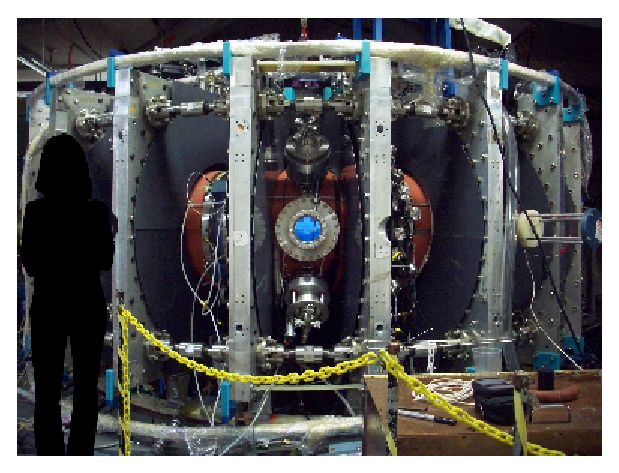
\includegraphics[width=0.8\hsize]{eps/tokamak.eps}
 \caption{The HBT-EP ``Tokamak'' at Columbia University.}
 \label{fig:tokamak}
\end{figure}

Plasma control for fusion is an applications of energy CPS, where
complex algorithms must be computed at a very high rate.
Figure~\ref{fig:tokamak} shows the HBT-EP Tokamak at Columbia
University~\cite{Maurer_PPCF11,Rath_FED12} that magnetically controls
the 3-D perturbed equilibrium state of the plasma~\cite{Boozer_PP99}.
It is required to process 96 inputs and 64 outputs of 16-bit data at a
sampling rate of a few microseconds.
An initial attempt of the Columbia team employed fast CPUs or FPGAs, but
even the simplified algorithm failed to run within 20$\mu$s.
An alternative approach was to parallelize the algorithm for the
graphics processing unit (GPU) using CUDA~\cite{CUDA}, the most
successful massively parallel computing technology.
However, the current system for GPU computing is not designed to
integrate sensor and actuator devices.
This is largely attributed to the fact that the GPU computing stack is
independent of I/O device drivers.
Since it may take tens of microseconds to transfer hundreds of bytes
between the CPU and the GPU, the current system does not allow plasma
control to use the GPU.
This is a signficant problem not only for plasma control but also for
many applications of CPS that utilize compute devices with I/O devices.

To the best of our knowledge, there is currently no generic support for
direct communication between the GPU and I/O devices, though a
specialized proprietary product for InfiniBand networks is
available~\cite{GPUDirect}.
There are also pinned memory allocation methods available from current
programming frameworks to reduce data-copy operations, but it is unclear
if they are best suited for real-time GPU applications. 
Although GPUs have been increasingly utilized in the domain of
CPS~\cite{Hirabayashi_REACTION12, Mangharam11, McNaughton_ICRA11,
Michel_IROS07}, and GPU resource management techniques have been
invented~\cite{Elliott_RTS12, Elliott_ECRTS12, Kato_RTAS11, Kato_RTSS11,
Kato_ATC11, Kato_ATC12, Liu_PACT12}, an integration of I/O processing
and GPUs remains an open problem.

In this paper, we present a zero-copy I/O processing scheme for GPU
applications.
This scheme incorporates functions and their application programming
interface (API) for I/O device drivers to directly transfer data to and
from GPU memory space, removing additional data-copy operations between
the CPU and the GPU.
We also investigate exisiting approaches, and compare them to the
presented zero-copy I/O processing scheme.
Our case study uses the Columbia University's Tokamak plasma control
system to evalaute a reduced sampling rate of plasma control.
In order to evaluate more generic properties of I/O processing schemes,
we further provide microbenchmarks, and discuss the pros and cons of each
scheme.
By clarifying GPU capabilities, we aim to not only improve the overall
performance but also broaden the scope of CPS that can benefit from the
use of GPU technology.



\section{Case Study}
\label{sec:case_study}

In this section, we provide a case study of magnetic control of
perturbed plasma equilibria using the HBT-EP ``Tokamak'' equipped with
the GPU and the presented I/O processing schemes.
This control system requires low latency and high computing capabilities
to achieve a sampling period of the order of ten microseconds, while
processing 96 inputs and 64 outputs of 16-bit data with a complex
algorithm.
As mentioned in Section~\ref{sec:introduction}, the CPU implementation
of this algorithm has never met the requirement of computing power.
The case study presented herein, therefore, is significant in that we look
into a possibility of GPU implementations for the plasma control system.

\begin{figure}[t]
 \centering
 \includegraphics[width=\hsize]{eps/tokamak_sysarch.eps}
 \caption{HBT-EP magnetic sensors and control coils connected with the
 GPU.}
 \label{fig:tokamak_sysarch}
\end{figure}

Figure~\ref{fig:tokamak_sysarch} shows a system architecture used in
this case study.
The control input comes from a set of magnetic sensors through a D-TACQ
ACQ196 digitizer, and the resulting control signal is sent to two D-TACQ
AO32 analog output modules to excite control coils.
These input and output modules are connected to the GPU upon the PCIe
bus.
We evaluate three different schemes against this system architecture
from the viewpoint of the cycle time of algorithm execution and the
latency of data transfer. 
Each scheme is applied as follows:
\begin{itemize}
 \item In the {\hd} scheme, the device driver of the digitizer transfers
       the input data set to the buffers allocated on the host memory.
       The control program copies this data set to the device memory via
       PCI-mapped host memory space, and the parallelized control
       algorithm runs on the GPU with the data on the device memory.
       Once the output data set is produced by the GPU, the control
       program copies it back to the host memory, and it is finally
       pulled by the device driver of the analog output modules.
       This is the traditional form of GPU computing.
 \item The {\hp} scheme pins the input and output buffers to PCI-mapped
       host memory space.
       Since the data set pushed and pulled by the device drivers of
       the I/O modules is directly accessible to the GPU, there is no
       need to perform data copies.
       However, this scheme must compromise the latency of data access
       imposed on the GPU when executing the control algorithm.
 \item Similarly to the {\hp} scheme, the {\dm} scheme proposed in this
       paper uses pinned PCI-mapped host memory space to allocate the
       input and out buffers, and further maps it to the device memory
       through PCI BAR space.
       Thus, there is no need of data copies while the data access of
       the control algorithm is limited within the device memory.
\end{itemize}

\begin{figure}[t]
 \centering
 \includegraphics[width=\hsize]{eps/eval_plasma.eps}
 \caption{Cycle time and latency of the plasma control system.}
 \label{fig:eval_plasma}
\end{figure}

We now demonstrate that our zero-copy I/O processing scheme reduces both
the cycle time of algorithm execution and the latency of data transfer
in this control system.
Figure~\ref{fig:eval_plasma} shows the result of experiments conducted
under the three different schemes, respectively.
Apparently, the {\dm} scheme achieves the highest rate in both algorithm
execution and data transfer.
The remaining two schemes, on the other hand, compromise either of them.
It is fairly reasonable to observe that the {\hd} and the {\dm} schemes
exhibit the same performance level for algorithm execution since they
both use the device memory, while the latency of data transfer is
equivalent between the {\hp} and the {\dm} schemes since they both
remove data copies.
Comparing the {\hd} and the {\hp} schemes, one can also observe that the
impact of overhead introduced by data copies, \textit{i.e.}, $16\mu$s, is
greater than that introduced by the GPU accessing pinned host memory
space, \textit{i.e.}, $6\mu$s, on the overall system performance.
Curiously, there is additional latency of $4\mu$s observed when running
the control system.
We suspect that this latency comes from some interactions among the host
computer, the graphics card, and the I/O modules.
Lessons learned from this evaluation are summarized as follows:
\begin{itemize}
 \item Zero-copy I/O processing is very effective for this control
       system, reducing the latency of data transfer from $16\mu$s to
       $4\mu$s.
       The speed-up ratio is 4$\times$.
 \item Furthermore, the {\dm} scheme proposed in this paper reduces the
       cycle time of algorithm execution from $6\mu$s to $4\mu$s.
       The speed-up ratio is 1.5$\times$.
       Since the HBT-EP ``Tokamak'' accommodates up to 216 inputs,
       meaning that the cycle time of algorithm execution is more
       dominated by data accesses, the benefit of the {\dm} scheme over
       the {\hp} scheme would be more significant for a larger scale of
       plasma control.
\end{itemize}

\begin{figure}[t]
 \centering
 \includegraphics[width=0.85\hsize]{eps/oscilloscope.eps}
 \caption{Screenshot of the oscilloscope.}
 \label{fig:oscilloscope}
\end{figure}

The above measurement explains that the control system can operate at a
sampling period of $16\mu$s.
The data transfer from and to the input and output modules takes $4\mu$s
each.
The algorithm execution takes $4\mu$s.
Adding additional latency of $4\mu$s, the total control rate must be
able to achieve $16\mu$s.
Figure~\ref{fig:oscilloscope} depicts the screenshot of the oscilloscope
where we measure the signals of the input and the output modules.
The topmost and middle signals represent the input and the output,
respectively, while the lower signal indicates the base clock.
The grid spacing of the X axis is $5\mu$s.
The time interval from the first downward edge in the clock signal after
the input signal goes up to the instant when the output signal starts
uprising is almost equal to $16\mu$s.
This means that the total control processing time is $16\mu$s. 

We next demonstrate that the control system is running properly at a
rate of $16\mu$s.
The control input comes from a set of magnetic sensors arranged in a
ring, as illustrated in Figure~\ref{fig:tokamak_sysarch}, and the
magnetic field that they measure is rotating, whose orientation is
described by a \textit{phase}.
Ideally, the phase is equivalent to multiplication of time and
frequency.
To control this mode, the control system needs to produce a control
signal that generates an equal and opposite field, which also needs to
rotate.
Obviously, the two fields should have a constant phase difference,
because it is given by multiplication of the control processing time and
the rotation frequency.
However, in practice, the rotation frequency is not constant but is
changing.
As a result, the phase difference appears to oscillate, with the base
output signal, which can be found as spikes in
Figure~\ref{fig:phase_base}.
Now, we measure the phase difference with the output signal time-shifted
by $16\mu$s.
In other words, the effective control system latency is reduced by
$16\mu$s.
As shown in Figure~\ref{fig:phase_shifted}, the spikes are now all
removed.
This indicates that the control system is perfectly in phase with the
mode, and the effective control system latency now must be zero,
\textit{i.e.}, the actual latency is $16\mu$s.

\begin{figure}[t]
 \centering
 \includegraphics[width=0.7\hsize]{eps/75221_base.eps}
 \caption{Phase difference observed with the base output signal.}
 \label{fig:phase_base}
\end{figure}
\begin{figure}[t]
 \centering
 \includegraphics[width=0.7\hsize]{eps/75221_shifted.eps}
 \caption{Phase difference observed with the output signal shifted by 16$\mu$s.}
 \label{fig:phase_shifted}
\end{figure}

\begin{figure}[t]
 \centering
 \includegraphics[width=0.9\hsize]{eps/overview.eps}
 \caption{Practical findings of plasma control.}
 \label{fig:plasma_overview}
\end{figure}

Finally, we discuss practical findings of plasma control regarding the
HBT-EP ``Tokamak'' device.
Figure~\ref{fig:plasma_overview} shows a comparison of the average
perturbation amplitudes with different phasings.
The control system incorporates four arrays of magnetic sensors and
control coils, each of which controls one specific mode.
They are placed at different poloidal angles around the toroidal ring.
Due to their different locations, they measure slightly different
amplitudes.
From this experiment, we find that feedback at 280 degrees excites
perturbation, while feedback at 100 degrees is the right range for
suppression.
As compared to no feedback scenario (``No FB'' in the figure), for
example, we find that we can supress the strength of the rotating field
by up to 30\% for any mode observed in this experiment.
\section{Benchmarking}
\label{sec:benchmarking}

We now evaluate generic properties of the presented I/O processing
schemes.
To do so, we remove constraints of I/O devices, and focus on naive
microbenchmarking programs of matrix operations performing with the host
and the device memory.
In particular, timing analysis of addition and multiplication of varying
sized matrices is conducted.
These programs are considered as the most basic parallel computing
programs also used in prior work~\cite{Rossbach_SOSP11}.
Since our focus is on data access and I/O processing, but not on
computation, we choose matrix addition as a microbenchmark, as it is 
a straightforward operation for the GPU.
Matrix multiplication, on the other hand, is also included to briefly
illustrate how an increase of computational complexity and data accesses
affects time to completion.
We also showcase effective host read and write throughput for each I/O
processing scheme.
This benchmarking clarifies the capabilities of the presented scheme, not
specific to plasma control but applicable to generic low-latency
GPU computing.

The microbenchmarking experiments are conducted using the NVIDIA Quadro
5000 GPU (448 cores and 2.5GB memory), which is more end-user oriented
than the Tesla C2050 used in the case study.
Note that the supported number of compute cores is the same between
these two GPUs.

\subsection{Matrix Operations}
\label{sec:matrix}

We first demonstrate performance details of matrix operations.
To highlight the details, we use a large size of $2048\times2048$ matrix
in this experiment.
The properties of operations focused on are listed as follows:

\begin{itemize} \itemsep1pt
 \item {\bf Init:} GPU initialization time.
 \item {\bf MemAlloc:} Memory allocation time, with respect to the host
       and/or the device memory.
 \item {\bf DataInit:} Matrix initialization time.
 \item {\bf HtoD:} Copy time from the host to the device memory (only \hd).
 \item {\bf Exec:} Execution time of the kernel function.
 \item {\bf DtoH:} Copy time from the device to the host memory (only
       \hd\ and \dmh).
 \item {\bf DataRead:} Access time to read the result.
 \item {\bf Close:} Context destroying time.
\end{itemize}

\begin{figure}[t]
\centering
\includegraphics[width=0.5\textwidth, trim=0.0in 3.25in 0.0in 0.25in,
 clip=true]{eps/madd_time_spent.eps}
\caption{Details of matrix addition.}
\label{fig:madd_time_spent}
\end{figure}
\begin{figure}[t]
\centering
\includegraphics[width=0.5\textwidth, trim=0.0in 3.0in 0.0in 0.5in,
 clip=true]{eps/mmul_time_spent.eps}
\caption{Details of matrix multiplication.}
\label{fig:mmul_time_spent}
\end{figure}
\begin{figure}[t]
\centering
\includegraphics[width=0.5\textwidth, trim=0.0in 2.0in -0.3in 0.74in,
 clip=true]{eps/madd_time.eps}
\caption{Total matrix addition times.}
\label{fig:madd_time}
\end{figure}
\begin{figure}[t]
\centering
\includegraphics[width=0.5\textwidth, trim=0.0in 2.0in -0.3in 0.72in,
 clip=true]{eps/mmul_time.eps}
\caption{Total matrix multiplication times.}
\label{fig:mmul_time}
\end{figure}

Figure \ref{fig:madd_time_spent} shows where the system spends its time
in performing a $2048\times2048$ integer matrix addition using each of
the four schemes.
First, it is clear from Figure \ref{fig:madd_time_spent} that using our
{\dmh} scheme the total time to completion is less than the others, 
almost $34\%$ less than its nearest competitor, \textit{i.e.}, the {\hd}
scheme.

A more interesting observation is the comparison of how much
time is spent for each sub-task.
For most time categories, the {\dmh} scheme seems to enjoy the best of
each of the other three.
The memory allocation time for the {\dmh} scheme is nearly
identical to that of the {\hd} and the {\dm} schemes, and clearly less
than the {\hp} scheme.
The same is true for the execution times. 
Similarly, for data initialization, the {\dmh} scheme is just as good as
the {\hp} and the {\dm} scheme, which are superior to the {\hd} scheme.

The most notable difference among the four schemes is the data read time
for the {\dm} scheme, which is orders-of-magnitude greater than the
rest.
A $2048\times2048$ integer matrix represents 16MB of data, and the {\dm}
scheme reads 4 bytes at a time across the PCIe bus.
This was the motivation for our \dmh\ scheme.
Instead of reading one matrix element at a time, the {\dmh} scheme first
copies the data to the host before reading.
This evinces that the {\dm} scheme may suffer from a large size of data,
while it was very effective for the case study presented in
Section~\ref{sec:case_study} that deals with 96 inputs and 64 outputs of
16-bit data, \textit{i.e.}, 2KB of data.

The same anomaly is present in the execution time for the {\hp} scheme
-- the GPU must read one element at a time from the host memory, while
in the other three schemes the data reside on the GPU during
computation.
This makes the {\hp} scheme increasingly inferior as the data size
grows.

Figure \ref{fig:mmul_time_spent} shows the same time analysis for matrix
multiplication.
The only difference appears in the execution times.
This is not surprising as the multiplication experiments are exactly the
same as the addition ones except for the kernel function on the GPU.
In fact, if execution times are omitted, Figures
\ref{fig:madd_time_spent} and \ref{fig:mmul_time_spent} would look
almost identical.
This observation implies that the zero-copy I/O processing schemes are
not really appreciated by strongly compute-intensive applications.

While the above experiments do present a real-world scenario, in a
real-time system it is more likely that tasks are performed repeatedly,
and therefore the GPU initialization and closing costs might occur only
once -- the same context loaded a priori would remain active while only
the data might change.
In addition, it could be the case that the memory allocated for the task
could be reused, and only the contents modified.
For these reasons, the remainder of our analysis focuses only on read,
write, transfer, and execution. 

Figure~\ref{fig:madd_time} shows the time to completion of matrix
addition as a function of matrix size at the logarithmic scale.
The {\hp} scheme appears to be the best performer until a matrix size of
$32\times32$, corresponding to a data size of 4KB for each matrix, at
which point the {\dmh} becomes superior.
This is also reflected in the matrix multiplication times, as shown in
Figure~\ref{fig:mmul_time}. 
One thing to note is the growth rate of the {\hp} in matrix
multiplication; since each thread must perform multiplication and
addition $n^2$ times, as compared with one addition in matrix addition,
the number of reads that occur across the PCIe bus increases by a
greater exponential factor.
We expect that the time for the {\hp} scheme would eventually surpass
the {\dm} scheme, as the trend in the graph indicates.

%Note that even with the logarithmic time scale the curves appear exponential because while the matrix length and width increase as $2^n$ the data size of the
%matrix is $2^n \times 2^n \times 4 =  2^{2n+2}$ bytes (for 32-bit integers).

\subsection{Data Throughput}
\label{sec:data_throughput}

Finally, we evaluate the data throughput of the presented I/O processing
schemes, independent of computational units.
In other words, this evaluation shows the pure performance of data
communication between the host and the device memory.
We use the term ``effective throughput'' to mean ($size/time$) where
$time$ is measured from the beginning of data initialization to the
point at which it is actually available to the GPU.
For example, in the case of the {\hd} scheme, this corresponds to the
total time for the host processor to write to each element in the data
structure, which is in the host memory, plus the time to copy the data
to the device memory.

Figure~\ref{fig:write_tput} shows that the write throughput of the
{\dmh} is better than the {\hd} scheme by about a factor of 2 and at
least as good as the others, which all coincide almost exactly in the
graph.
Meanwhile, Figure~\ref{fig:read_tput} paints a slightly different
picture for read throughput.
It should not be surprising that the {\hp} scheme outperforms the rest
as it represents the host iterating over a data structure that is
already in the host memory.
The {\hd} and the {\dmh} schemes, on the other hand, must first copy the
data from the device to the host memory, and they achieve roughly equal
performance.
Note that they coincide in the graph.
Finally, the {\dm} scheme is the weakest performer due to a large
number of small reads that occur across the PCIe bus.

\begin{figure}[t]
\centering
\includegraphics[width=0.5\textwidth, trim=0.0in 2.75in -0.1in 0.60in,
 clip=true]{eps/write_tput.eps}
\caption{Host write throughput.}
\label{fig:write_tput}
\end{figure}
\begin{figure}[t]
 \centering
 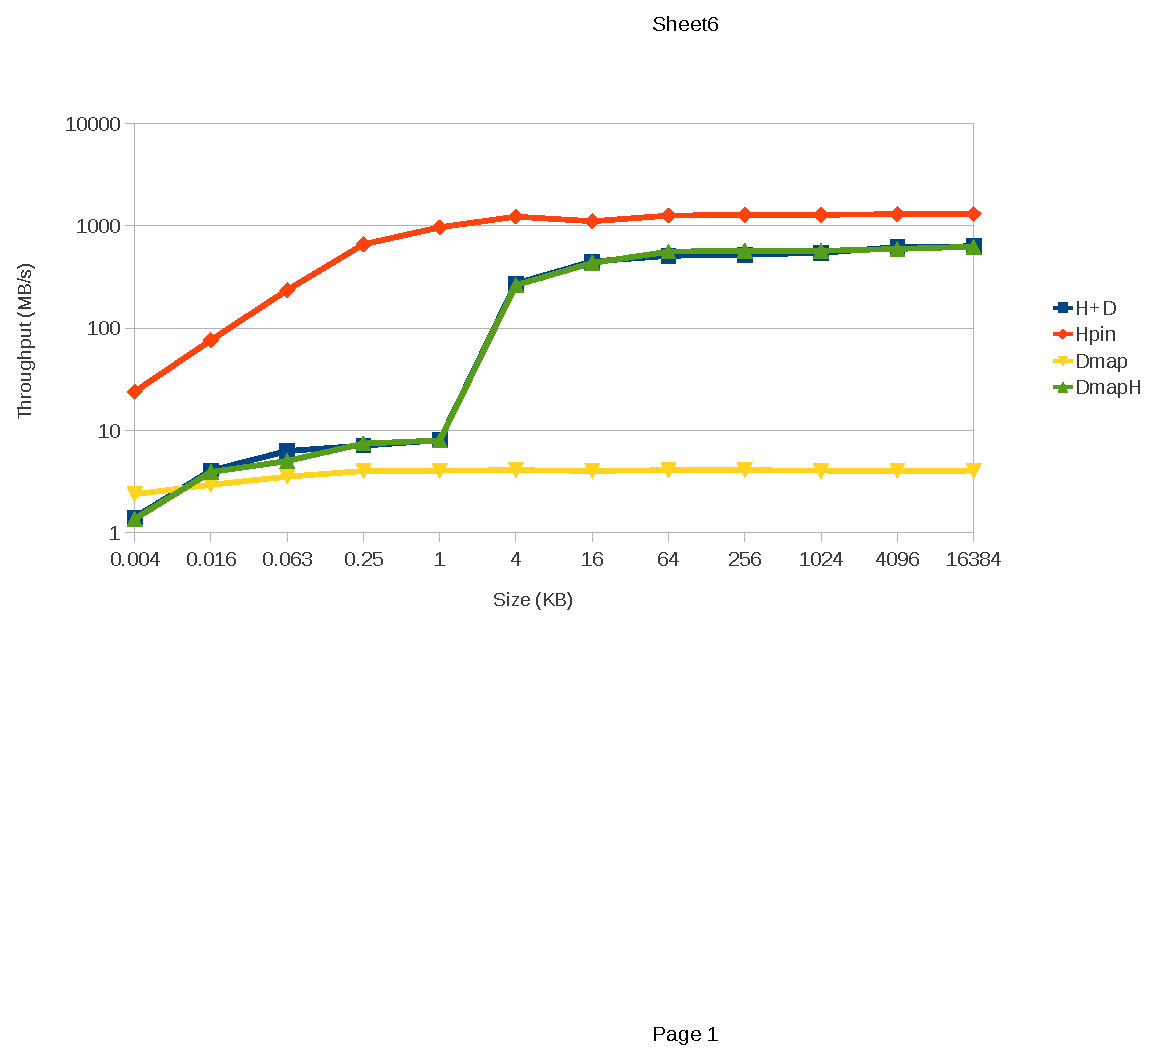
\includegraphics[width=0.5\textwidth, trim=0.0in 2.5in -0.1in 0.6in,
 clip=true]{eps/read_tput.eps}
 \vspace{-2em}
 \caption{Host read throughput.}
\label{fig:read_tput}
\end{figure}


\bibliographystyle{abbrv}
\bibliography{references}

\end{document}
